% To convert to svg
% lualatex --output-format=dvi filename.tex
% dvisvgm filename.dvi
%\documentclass[a3paper]{article}
%\usepackage[left=0mm,top=1cm,right=0mm,bottom=0mm]{geometry}
% \documentclass[border=0]{standalone}
\documentclass[dvisvgm]{minimal}
\usepackage{tikz}
\usetikzlibrary{calc}
\usepackage{xcolor}
% \definecolor{pGreen}{HTML}{006633}
% \definecolor{pRed}{HTML}{cc0033}

\begin{document}
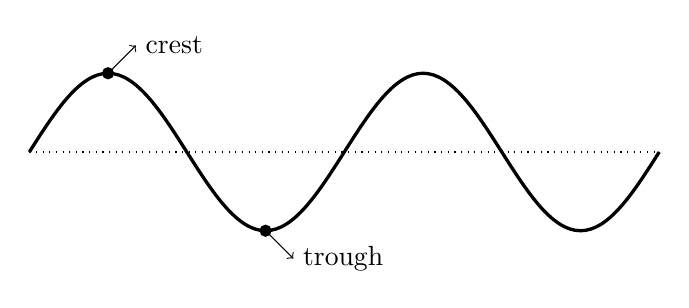
\begin{tikzpicture}
    % \clip (1,-1) rectangle (7,1);
    \pgfmathsetmacro{\w}{1}	%scale
	\pgfmathsetmacro{\a}{4}
	\pgfmathsetmacro{\b}{1}

    \draw[dotted] (0,0) -- (8,0);
    \draw[very thick] (0,0) sin (1,1) cos (2,0) sin (3,-1) cos (4,0) sin (5,1) cos (6,0) sin (7,-1) cos (8,0);
    \filldraw (1,1) circle [radius=2pt];
    \draw[->] (1,1) --++(45:.5) node[right] {crest};
    \filldraw (3,-1) circle [radius=2pt];
    \draw[->] (3,-1) --++(-45:.5) node[right] {trough};
\end{tikzpicture}
\end{document}
